From the given information, 
for
\begin{align}
\vec{u} = \myvec{u_1\\u_2}\succeq \vec{0},
\end{align}
%
the given conditions can be expressed as
\begin{align}
\myvec{1 & 0 \\ 0 & 1}\vec{x}  &\succeq \myvec{3\\2}
\\
\implies \myvec{1 & 0 \\ 0 & 1}\vec{x}  -\vec{u}&=\myvec{3\\2}
\\
\text{or, }
\myvec{1 & 0 \\ 0 & 1}\vec{x} &= \myvec{3\\2} +\vec{u}
\end{align}
%
resulting in 
\begin{align}
\vec{x} &= \myvec{1 & 0 \\ 0 & 1}^{-1}\myvec{3\\2} +\myvec{1 & 0 \\ 0 & 1}^{-1}\vec{u}
\\
\text{or, } \vec{x} &= \myvec{3\\2} +\myvec{1 & 0 \\ 1 & 0}\vec{u}
\end{align}
%
after obtaining the  inverse.
%
 Fig. \ref{fig:3.11.1_line_ineq} generated using the following python code shows the desired region 

\begin{lstlisting}
solutions/1/codes/line/line_eq.py
\end{lstlisting}
%
\begin{figure}[!ht]
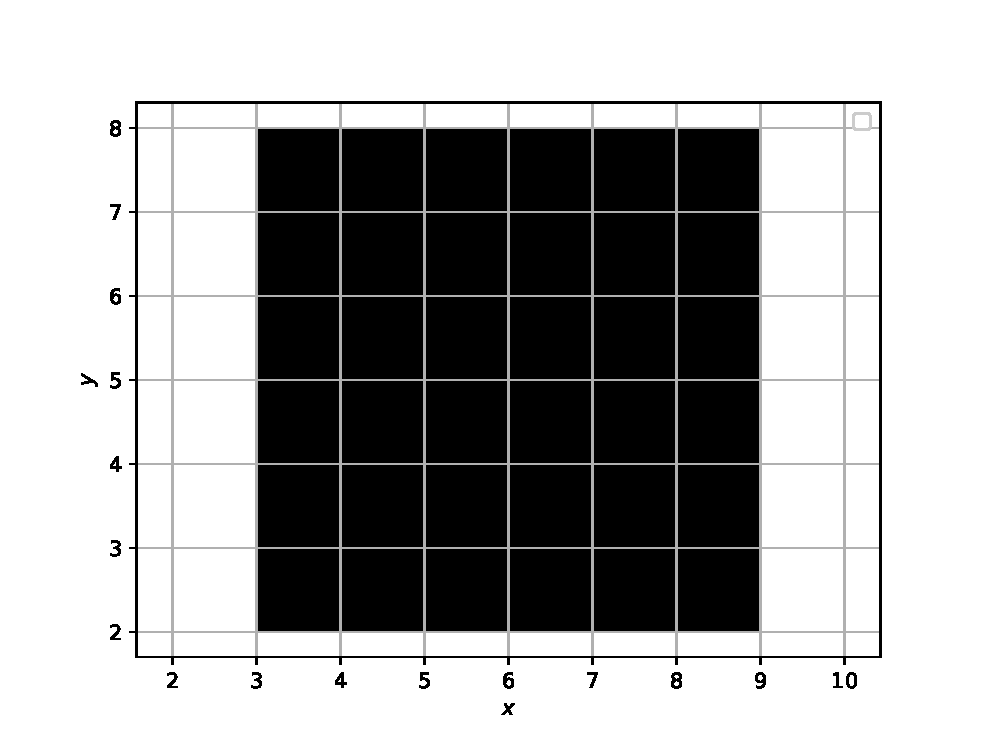
\includegraphics[width=\columnwidth]{./solutions/1/figs/line/line_eq.eps}
\caption{}
\label{fig:3.11.1_line_ineq}
\end{figure}
%



